\begin{figure}[H]
    \centering
    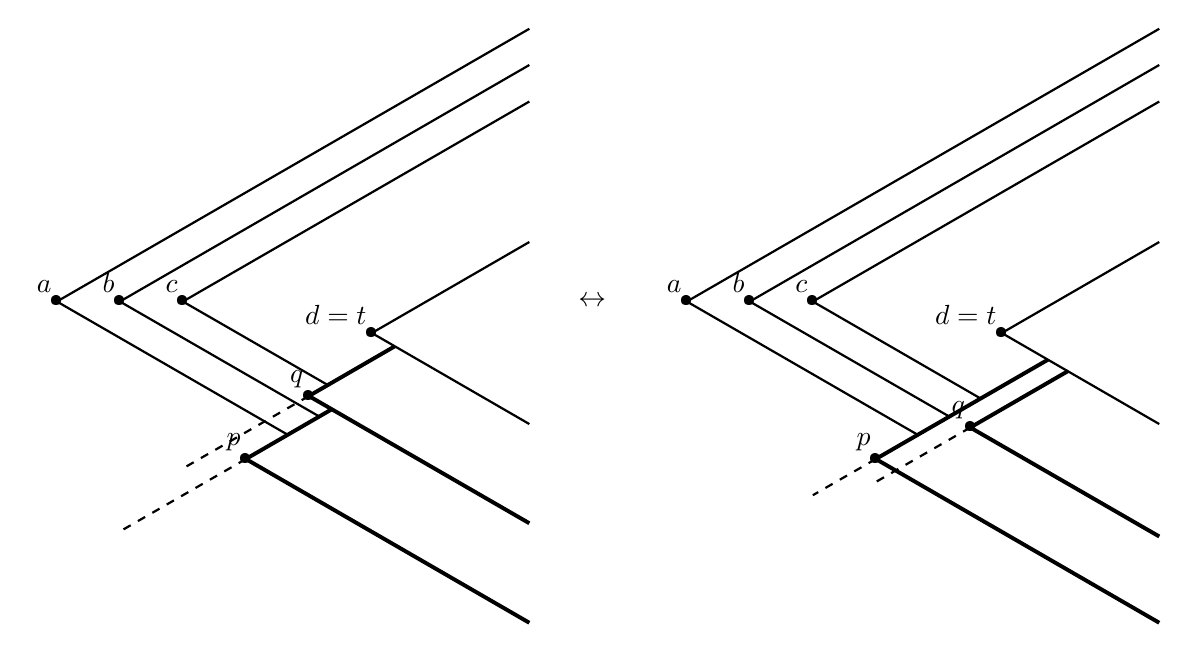
\begin{tikzpicture}[thick, scale=0.4]
        \node[label={[label distance = -3mm]160:$p$}] at
        (6.00, 0.00) {\textbullet};
        \node[label={[label distance = -3mm]160:$q$}] at
        (8.00, 2.00) {\textbullet};
        \node[label={[label distance = -3mm]160:$a$}] at
        (0.00, 5.00) {\textbullet};
        \node[label={[label distance = -3mm]160:$b$}] at
        (2.00, 5.00) {\textbullet};
        \node[label={[label distance = -3mm]160:$c$}] at
        (4.00, 5.00) {\textbullet};
        \node[label={[label distance = -3mm]160:$d = t$}] at
        (10.00, 4.00) {\textbullet};

        % d cone
        \draw (10.00, 4.00) -- (15.00, 1.11);
        \draw (10.00, 4.00) -- (15.00, 6.89);
        % q cone
        \draw[dashed] (8.00, 2.00) -- (4.00, -0.30);
        \draw[line width = 0.5mm] (8.00, 2.00) -- (15.00, -2.04);
        \draw[line width = 0.5mm] (8.00, 2.00) -- (10.73, 3.58);
        % p cone
        \draw[dashed] (6.00, 0.00) -- (2.00, -2.30);
        \draw[line width = 0.5mm] (6.00, 0.00) -- (15.00, -5.20);
        \draw[line width = 0.5mm] (6.00, 0.00) -- (8.73, 1.58);
        % c cone
        \draw (4.00, 5.00) -- (8.60, 2.35);
        \draw (4.00, 5.00) -- (15.00, 11.35);
        % b cone
        \draw (2.00, 5.00) -- (8.33, 1.35);
        \draw (2.00, 5.00) -- (15.00, 12.51);
        % a cone
        \draw (0.00, 5.00) -- (7.33, 0.77);
        \draw (0.00, 5.00) -- (15.00, 13.66);

        \node at (17, 5) {$ \leftrightarrow$};

        \node[label={[label distance = -3mm]160:$p$}] at
        (26.00, 0.00) {\textbullet};
        \node[label={[label distance = -3mm]160:$q$}] at
        (29.00, 1.00) {\textbullet};
        \node[label={[label distance = -3mm]160:$a$}] at
        (20.00, 5.00) {\textbullet};
        \node[label={[label distance = -3mm]160:$b$}] at
        (22.00, 5.00) {\textbullet};
        \node[label={[label distance = -3mm]160:$c$}] at
        (24.00, 5.00) {\textbullet};
        \node[label={[label distance = -3mm]160:$d = t$}] at
        (30.00, 4.00) {\textbullet};

        % d cone
        \draw (30.00, 4.00) -- (35.00, 1.11);
        \draw (30.00, 4.00) -- (35.00, 6.89);
        % q cone
        \draw[dashed] (29.00, 1.00) -- (26.00, -0.73);
        \draw[line width = 0.5mm] (29.00, 1.00) -- (35.00, -2.46);
        \draw[line width = 0.5mm] (29.00, 1.00) -- (32.10, 2.79);
        % p cone
        \draw[dashed] (26.00, 0.00) -- (24.00, -1.15);
        \draw[line width = 0.5mm] (26.00, 0.00) -- (35.00, -5.20);
        \draw[line width = 0.5mm] (26.00, 0.00) -- (31.46, 3.15);
        % c cone
        \draw (24.00, 5.00) -- (29.33, 1.92);
        \draw (24.00, 5.00) -- (35.00, 11.35);
        % b cone
        \draw (22.00, 5.00) -- (28.33, 1.35);
        \draw (22.00, 5.00) -- (35.00, 12.51);
        % a cone
        \draw (20.00, 5.00) -- (27.33, 0.77);
        \draw (20.00, 5.00) -- (35.00, 13.66);
    \end{tikzpicture}
    \caption{Da direita para a esquerda, $p$, que estava em $\Hits_{up}(q)$
        foi transferido para $\Hits_{up}(t)$ e todos os elementos em
        $\Hits_{low}(q)$ foram transferidos para $\Hits_{low}(p)$. Da esquerda
        para a direita, $p$, que estava em $\Hits_{up}(t)$, foi transferido para
        $\Hits_{up}(q)$ e os pontos à direita de $v$ em $\Hits_{low}(p)$ foram
        transferidos para $\Hits_{low}(q)$.}
    \label{fig:parcinetico:eventodowntnaoexiste}
\end{figure}